\section{Введение}

\subsection{Трассы исполнения} \label{sec:execution_traces}

\gls{trace} представляет собой упорядоченный набор записей о событиях: исполнениях инструкций, операциях с памятью, системных вызовах, сигналах и т. д., происходивших во время трассировочного запуска приложения.

Трассы исполнения применяются в индустрии для различных задач, таких как: микроархитектурный и макро анализ приложений, сбор профилей исполнения, отладка \cite{trace_checkpoint_for_dvfs,plc_behav_model_from_traces,atlantis_paper,pinplay,lisitsyn_disser}. В рамках данной работы рассмотрены трассы для RISC-архитектуры.

Трасса может содержать записи для нескольких потоков исполнения, однако для простоты в дальнейшем будем рассматривать только трассы исполнения с одним потоком. Описанное в данной работе решение нетрудно обобщается на трассы с произвольным числом потоков.

Будем называть \glsdisp{app_instr}{инструкцией приложения (статической инструкцией)} статическую машинную инструкцию, расположенную в памяти трассируемой программы. Записи трассы исполнения, отвечающие одному выполнению инструкции приложения назовем \glsdisp{trace_instr}{инструкцией трассы (динамической инструкцией)}. Далее, если не оговорено иное, под инструкцией понимается именно динамическая инструкция.

Рассматриваемые трассы исполнения содержат следующие основные виды записей:

\begin{itemize}
    \item Начальное регистровое состояние

    Содержит значения регистров общего назначения, векторных регистров и условных флагов в момент начала трассировки. Также такие записи используются для отображения состояния машины при переключениях контекста исполнения (обработка сигналов, изменение уровня привилегий).

    \item Исполнение инструкции

    Содержит информацию об исполнении инструкции: адрес, кодировку и номер инструкции в трассе. С данной записью могут быть ассоциированы обращения в память и записи в регистры (см. ниже).

    \item Обращение в память

    Содержит адрес, размер, данные и тип обращения (запись или чтение). Одна инструкция может иметь несколько ассоциированных с ней обращений к памяти. Данные для чтения из памяти соответствуют состоянию памяти \textbf{до} исполнения инструкции.

    \item Запись в регистр общего назначения

    Содержит идентификатор регистра и его значение \textbf{после} исполнения инструкции. Одна инструкция может иметь несколько ассоциированных с ней записей в регистры. Такие записи используются для отслеживания изменений регистров общего назначения системными (системные вызовы, чтения системных регистров) и другими инструкциями.
\end{itemize}

Изменения памяти, осуществляемые операционной системой (\gls{os}) или другими потоками исполнения будут отражены в трассе (в записях для рассматриваемого потока) только косвенно: при чтении памяти может быть прочитано новое значение, не соответствующее образу памяти, который наблюдался ранее. На рис. \ref{fig:trace_example} приведен пример трассы исполнения, в том числе иллюстрирующий данную особенность (см. записи 2 и 6).

\begin{figure}[h!]
    \centering
    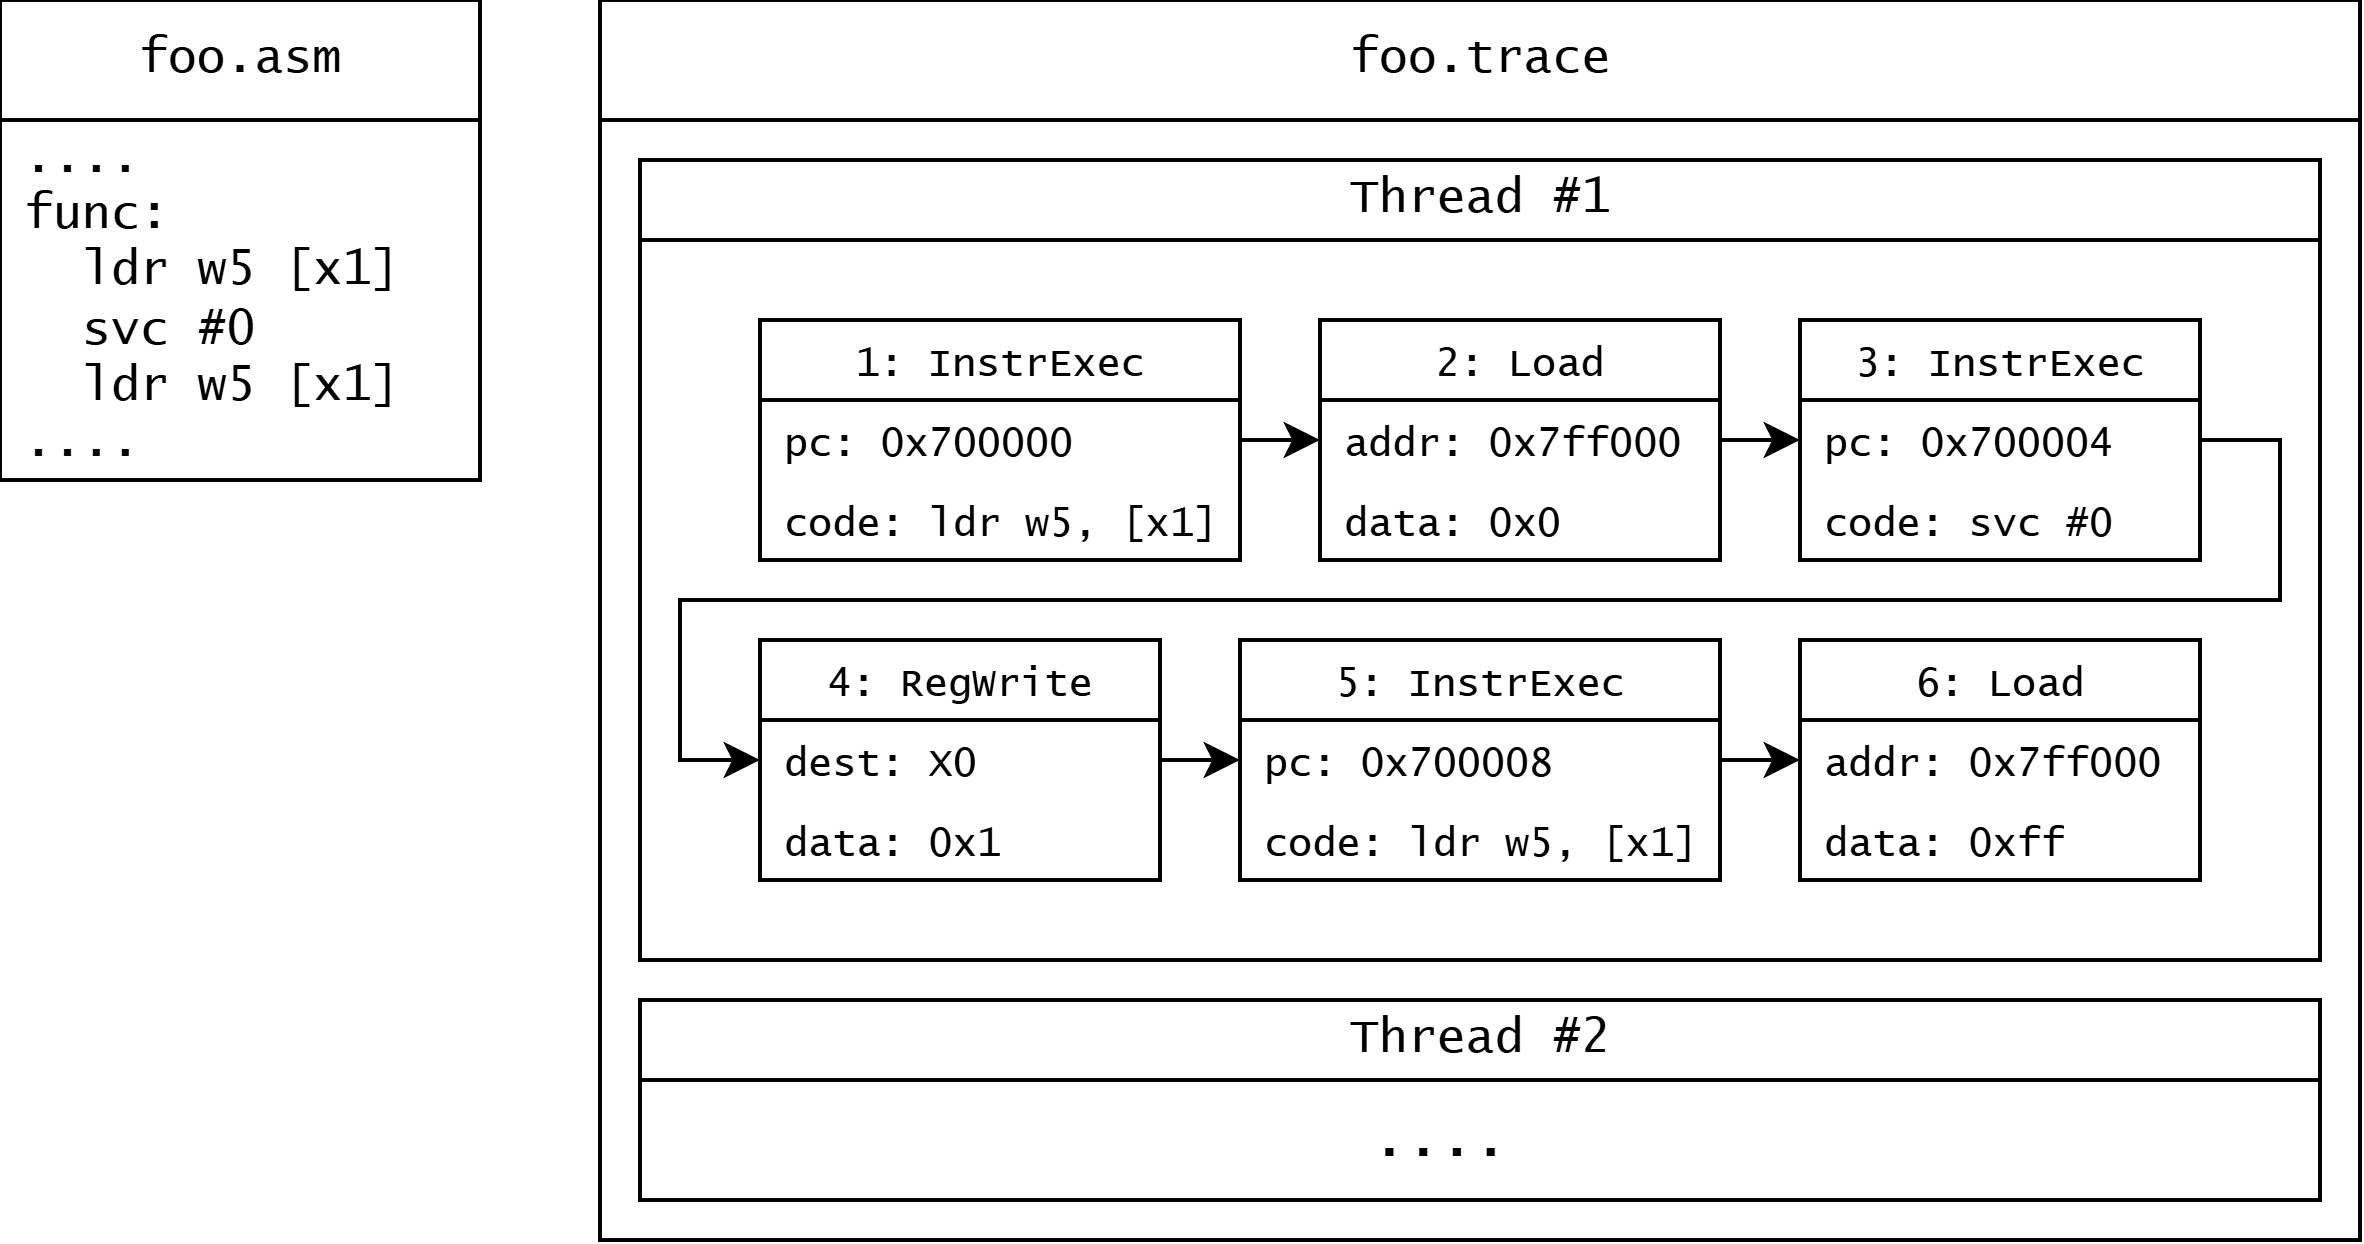
\includegraphics[width=0.8\linewidth]{pics/trace_example.drawio.png}
    \caption{Пример трассы исполнения.}
    \label{fig:trace_example}
\end{figure}

При анализе трасс исполнения часто используются симуляторы \cite{nocua_gem5_trace_driven,synchrotrace}. В таких случаях в состояние симулятора пробрасываются данные из трассы, для рассматриваемых трасс это: начальное регистровое состояние, коды инструкций, данные для чтений из памяти, новые значения регистров общего назначения. При этом зачастую потоки управления и данных симулятора проверяются на соответствие трассе для детектирования ошибок симуляции или невалидных трасс. Такой подход называется симуляцией по трассе.

Описанные особенности трасс исполнения и их обработки позволяют существенно модифицировать записанные сценарии и получать валидные трассы для дальнейшей обработки: можно изменить или добавить необходимые записи для коррекции потоков управления и данных. На рис. \ref{fig:trace_example_modified} приведен пример модифицированной трассы исполнения. Измененные данные выделены красным цветом.

\begin{figure}[h!]
    \centering
    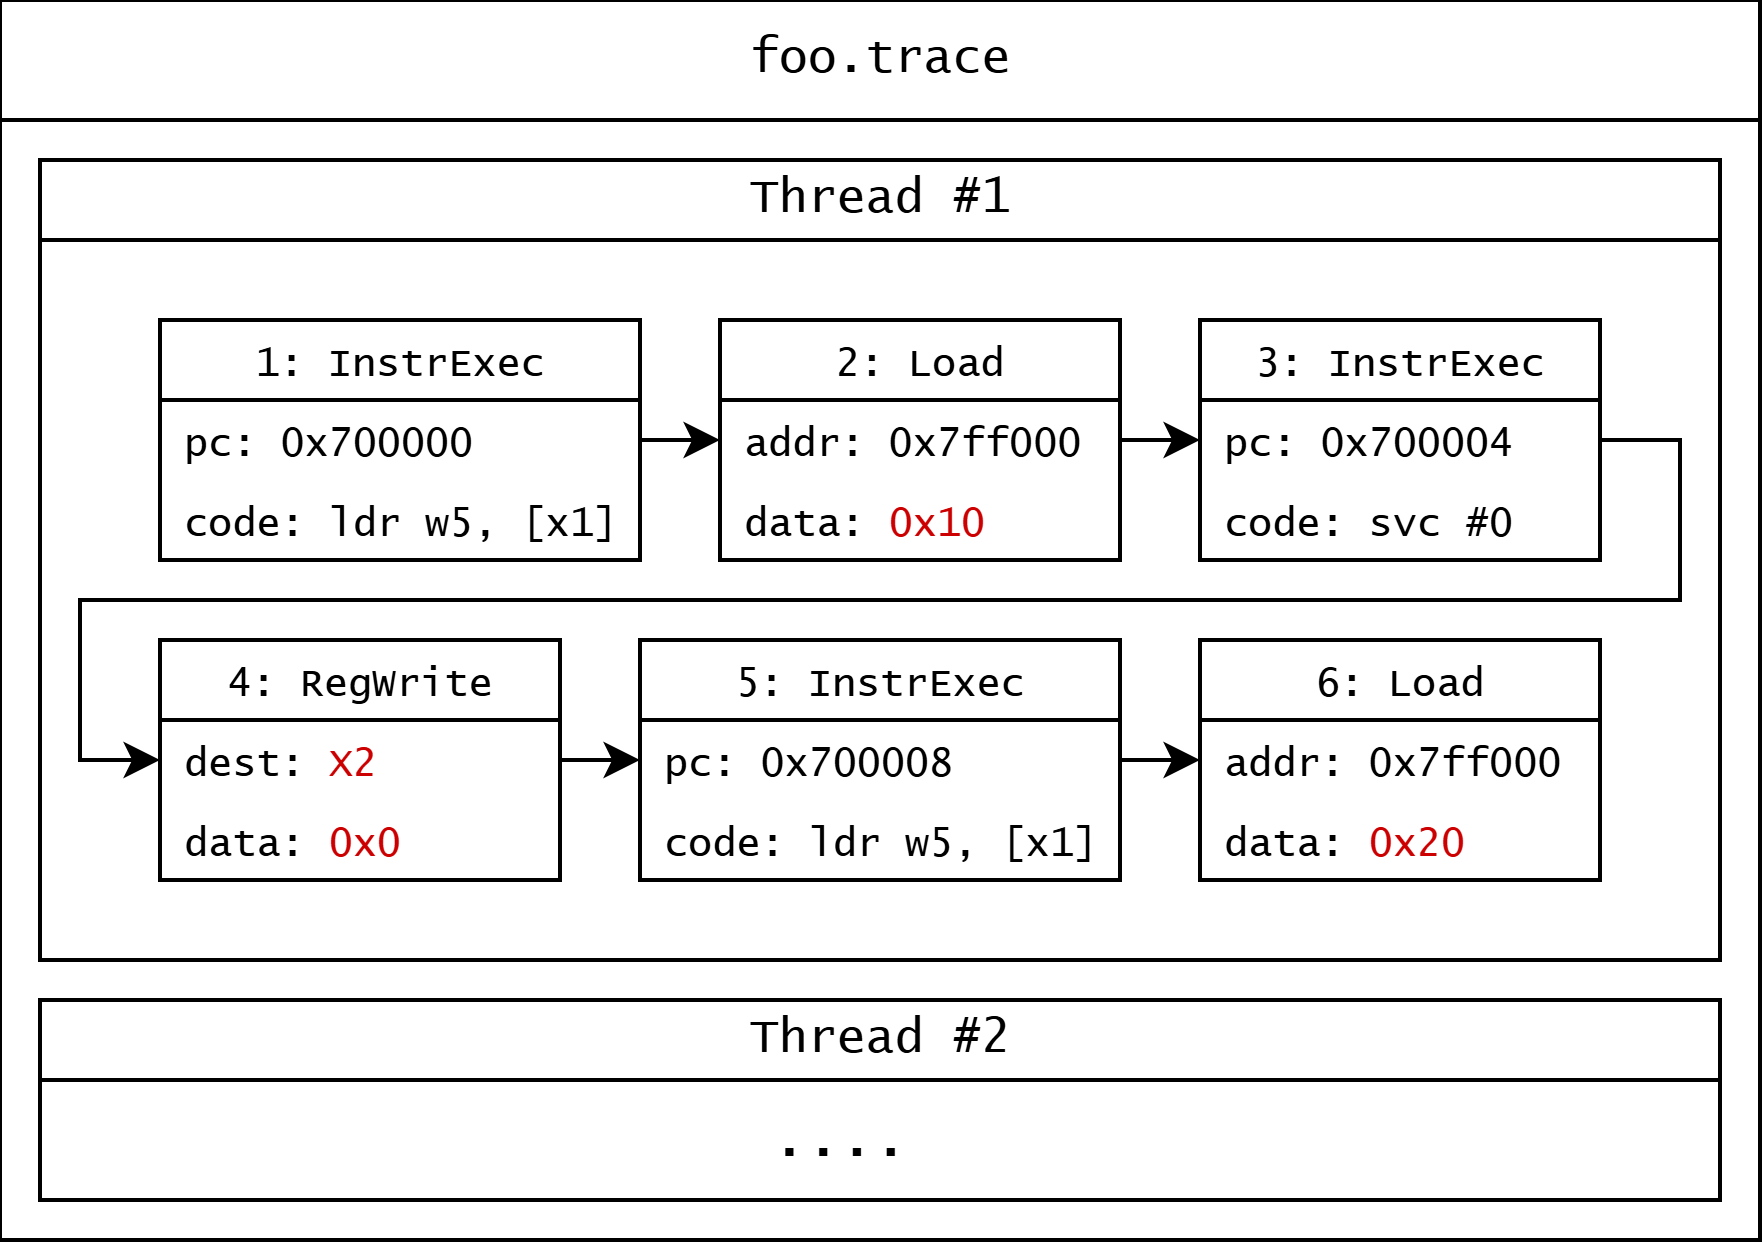
\includegraphics[width=0.6\linewidth]{pics/trace_example_modified.drawio.png}
    \caption{Пример модифицированной трассы исполнения.}
    \label{fig:trace_example_modified}
\end{figure}

\subsection{Репрезентативность трасс} \label{sec:representativeness}

Для оценки репрезентативности трасс обычно сличаются целевые метрики сценариев исполнения и метрики, получаемые при анализе трасс, снятых с этих сценариев. Значения могут расходиться по разным причинам: трассировка может влиять на поведение приложения; используемая модель или методы анализа трасс могут искажать получаемые значения; на исследуемую нагрузку могут влиять внешние факторы.

Как уже было упомянуто ранее, данная работа сфокусирована на использовании трасс исполнения для анализа производительности разрабатываемых платформ. Поэтому основными целевыми метриками являются значения микроархитектурных счетчиков. Для оценки репрезентативности сличаются счетчики, снятые с трассируемого приложения, и счетчики, полученные от используемой модели (сконфигурированной для симуляции трассируемой системы).

При обработке некоторых записей трассы исполнения симулятором или другой моделью появляется необходимость компенсации состояния модели. Пример: из памяти прочитано новое значение, которое ранее не наблюдалось -- требуется модификация памяти симулятора для корректного продолжения работы. Подобные изменения состояния модели производятся посредством исполнения дополнительного кода (далее -- компенсационный код), что может существенно искажать собираемые метрики. Более того, компенсационный код фиксирован для каждой инструкции приложения -- единожды произошедшая при симуляции инструкции трассы компенсация приводит к добавлению компенсационного кода для \textbf{всех} инструкций трассы, отвечающих той же инструкции приложения. Поэтому репрезентативность трасс исполнения существенно зависит от компенсаций, требуемых при обработке.

Подробно методология сбора микроархитектурных метрик и оценки репрезентативности трасс в данной работе рассмотрена не будет. Однако будут приведены метрики, используемые для предварительной оценки качества получаемых трасс.

\subsection{Виртуальное адресное пространство}

Большинство современных компьютерных систем поддерживает виртуализацию адресного пространства \cite{arm_memory_management}. Данная технология позволяет отображать (транслировать) адреса оперативной памяти, используемые кодом (виртуальные адреса) в адреса аппаратуры (физические адреса). Такой подход позволяет запускать множество приложений изолированно в одинаковой среде исполнения. Виртуальные адреса приложений могут пересекаться, однако при обращении к памяти будут использованы разные физические адреса. Создание карты трансляции адресов осуществляет операционная система по запросам приложений и загрузчиков.

При этом трансляция адресов обычно происходит постранично: виртуальное адресное пространство разбивается на непрерывные блоки одинакового размера (виртуальные страницы), последовательные адреса внутри одного блока отображаются в последовательные физические адреса (адреса физической страницы). Размер страницы - очень важный параметр системы, напрямую влияющий на производительность. Уменьшение размера страницы приводит к замедлению трансляции адресов, а увеличение - к большему расходу памяти. Типовые размеры страниц для современных систем: 4096, 16384 и 65536 байт.

К другим настройкам адресации можно отнести расположение запрещенных областей виртуального адресного пространства - областей, использование которых пользовательским кодом запрещено или ограничено. Такие области могут быть заняты данными операционной системы, зарезервированы для будущих расширений, запрещены для детектирования ошибок адресации (null page). Подобные области могут быть доступны из пользовательского кода только на чтение или недоступны вовсе.

Также многие современные системы имеют ограничения на создание отображений c правами на исполнение и запись (WX права) для повышения безопасности \cite{ye_executable_stack,openbsd_kernel_wx}.

\clearpage

\subsection{Цель работы}

Трассы исполнения могут быть использованы для анализа производительности еще не выпущенных платформ. Однако, описанные особенности виртуального адресного пространства существенно усложняют подобный анализ в случае, если настройки адресации разрабатываемой платформы отличаются от настроек адресации платформы, на которой трассы были записаны (исходные настройки адресации). Это мотивирует разработку решения для модификации образов памяти затрассированных сценариев путем изменения трасс исполнения. Заметим, что данная задача сводится к задаче перемещения областей образов памяти трасс в соответствии с новыми ограничениями.

\vspace{0.3cm}

{\bf Цель работы:} Разработать решение, позволяющее перемещать области образов памяти трассируемых сценариев в соответствии с ограничениями, обусловленными настройками адресации разрабатываемой платформы.

\vspace{0.3cm}

{\bf Задачи:}

\begin{itemize}
    \item Разработать модификатор трасс исполнения, перемещающий области образа памяти в соответствии с ограничениями, обусловленными новыми настройками адресации.
    \item Протестировать работоспособность модификатора трасс на целевых трассах заказчика.
    \item Оценить влияние модификаций на репрезентативность трасс исполнения.
\end{itemize}

Работа будет осуществляться в рамках проекта для сбора и анализа трасс исполнения. Будут использованы некоторые компоненты проекта, внешние по отношению к разрабатываемому решению: функциональный симулятор целевой архитектуры, библиотека для чтения и записи трасс исполнения.

\clearpage
